% use options
%  '[beamer]' for a digital projector
%  '[trans]' for an overhead projector
%  '[handout]' for 4-up printed notes
\documentclass[beamer]{beamer}

% change talk_preamble if you want to modify the slide theme, colours, and settings for trans and handout modes.
\newcommand{\pathtotrunk}{../}
\input{preamble.tex}
\usepackage{etex}
\usepackage{pgfpages}

%\usepackage{dcpic}
\usepackage{pictex}
\usepackage{pinlabel}
\usepackage{color}

\usepackage{tikz}
\usetikzlibrary{shapes}
\usetikzlibrary{backgrounds}
\usetikzlibrary{decorations.pathreplacing}
\usepackage{tikz-qtree}

% beamer mode
\mode<beamer>{
 \usetheme{CambridgeUS}
}

% transparency mode
\mode<trans>{
 \usetheme{CambridgeUS}
}

% handout mode
\mode<handout>{
 \usetheme{default}
 \setbeamercolor{background canvas}{bg=black!5}
 \pgfpagesuselayout{4 on 1}[letterpaper,landscape,border shrink=2.5mm]
}

\newcommand{\return}[2]{\hyperlink{#1}{\beamerreturnbutton{#2}}}
\newcommand{\goto}[2]{\hyperlink{#1}{\beamergotobutton{#2}}}
\newcommand{\skipto}[2]{\hyperlink{#1}{\beamerskipbutton{#2}}}


% This switches fonts to the Palatino family.
%  \renewcommand{\familydefault}{ppl}

\usepackage{array}

\renewcommand{\pathtodiagrams}{../diagrams/}

%\renewcommand{\bigraph}[1]{{\hspace{-3pt}\begin{array}{c}%
%  \raisebox{-2.5pt}{\includegraphics[height=6mm]{../../graphs/\hashlookup{#1}}}% 
%\end{array}\hspace{-3pt}}}


\usetikzlibrary{matrix}
\usetikzlibrary{arrows,backgrounds,patterns,scopes,external,
    decorations.pathreplacing,
    decorations.pathmorphing
}

\newlength{\fuzzwidth}
\setlength{\fuzzwidth}{2.5pt}
\newlength{\arrowlength}
\setlength{\arrowlength}{8pt}
\newlength{\arrowwidth}
\setlength{\arrowwidth}{.75pt}
\newlength{\pointrad}
\setlength{\pointrad}{1.5pt}
\newlength{\linewid}
\setlength{\linewid}{1.5pt}
\newlength{\circlerad}
\setlength{\circlerad}{16pt}
\newlength{\smcirclerad}
\setlength{\smcirclerad}{8pt}
\newcommand{\fillcolor}{black!60}
\newcommand{\fuzzcolor}{black!25}
\newcommand{\arrowcolor}{black!25}

\tikzset{
        fuzzright/.style={
        preaction={draw,line width=\fuzzwidth,\fuzzcolor,decorate,decoration={curveto,amplitude=0,raise=-.5*\fuzzwidth}}},
        fuzzleft/.style={
        preaction={draw,line width=\fuzzwidth,\fuzzcolor,decorate,decoration={curveto,amplitude=0,raise=.5*\fuzzwidth}}},
        fuzzrightpre/.style={ %%% Doesn't work
        preaction={draw,line width=2pt,\fuzzcolor,decorate,decoration={curveto,amplitude=0,raise=-1pt,pre=moveto,pre length=12pt}}},
        fuzzleftpre/.style={ %%% Doesn't work
        preaction={draw,line width=2pt,\fuzzcolor,decorate,decoration={curveto,post=moveto,post length=32pt,amplitude=0,raise=1pt}}},        
        outstyle/.style={\arrowcolor, line width=\arrowwidth},
        linestyle/.style={line width=\linewid}
}

\newcommand{\ld}[1]
{{}^*{#1}}
\newcommand{\rd}[1]
{{#1}^*}
\newcommand{\ldd}[1]
{{}^{**}{#1}}
\newcommand{\rdd}[1]
{{#1}^{**}}
\newcommand{\ldddd}[1]
{{}^{****}{#1}}
\newcommand{\rdddd}[1]
{{#1}^{****}}



%\setbeameroption{previous slide on second screen=right}

\author[Noah Snyder]{Noah Snyder \\ \url{http://math.columbia.edu/~nsnyder}}
\title{$3$-dimensional topology and finite tensor categories}
\date{Joint Meetings}

\usepackage{multimedia}


\begin{document}

\frame{\titlepage}

\begin{frame}
       \frametitle{Outline}
       \tableofcontents
\end{frame}

\beamertemplatetransparentcovered 

\mode<beamer>{\setbeamercolor{block title}{bg=green!40!black}}

\beamersetuncovermixins 
{\opaqueness<1->{60}} 
{} 


\AtBeginSection[]
{
   \begin{frame}<beamer>
       \frametitle{Outline}
       \tableofcontents[currentsection]
   \end{frame}
}

\section{Radford's theorem}

\begin{frame}{Radford's theorem for Hopf algebras}

\begin{theorem}[Radford 75]
If $H$ is a finite dimensional Hopf algebra and $g \in H$ and $\alpha \in H^*$ are the distinguished grouplike elements, then:
$$S^4(x) = g (\alpha \rightharpoonup x \leftharpoonup  \alpha^{-1}) g^{-1}.$$
\end{theorem}

\

\begin{theorem}[Larson-Radford 87-88]
If $H$ is semisimple in characteristic $0$, then $S^2 = 1$.
\end{theorem}


\end{frame}

\begin{frame}{Radford's theorem for tensor categories}

\begin{theorem}[ENO 04]
If $\cC$ is a finite tensor category and $D \in \cC$ is the distinguished invertible object, then there's a canonical isomorphism of tensor functors
$$x^{****}  \rightarrow D \otimes x \otimes D^{-1}.$$
\end{theorem}

\

\begin{theorem}[ENO 04]
If $\cC$ is semisimple in characteristic $0$, then $D \cong 1$.
\end{theorem}

\

\begin{conj}[ENO 02]
If $\cC$ is semisimple then there's a monoidal isomorphism $x^{**} \rightarrow x$.
\end{conj}
\end{frame}

\begin{frame}{Goal of talk}
\begin{block}{Question:}
Why is there a nice canonical formula for the quadruple dual?  Why is the double dual more difficult?
\end{block}

\

\begin{block}{Answer:}
The double dual corresponds to the generator of $\pi_1(\mathrm{SO}_3) = \mathbb{Z}/2$
\end{block}

\

\begin{block}{Technique:}
Build a $3$-dimensional fully local TFT.  Joint work with Chris Douglas and Chris Schommer-Pries.
\end{block}
\end{frame}

\section{Big Picture}

\begin{frame}{Topological Quantum Field Theories}
\begin{block}{Informal Idea}
An $n$-dimensional TQFT is an invariant of $n$-manifolds which can be computed via cutting and pasting.
\end{block}

\begin{block}{Formal Definition}
A TQFT is a symmetric monoidal functor $$\cF:\mathrm{Bord}_n \rightarrow \mathrm{Vec}.$$
\end{block}


\begin{block}{In more detail}
\begin{itemize}
\item Closed $n-1$-manifolds are sent to vector spaces
\item $n$-manifolds with boundaries are sent to linear maps
\item Gluing goes to composition
\item Disjoint union goes to tensor product
\end{itemize}
\end{block}
\end{frame}

\begin{frame}{Local Topological Field Theories}
\begin{block}{Informal Idea}
It would be even better if we could cut up along lower dimensional pieces, and best of all if we could cut things up all the way down to points.
\end{block}

\

\begin{block}{Formal Definition}
An $n$-dimensional fully local topological field theory with values in a symmetric monoidal $n$-category $\cC$ is a symmetric monoidal functor:
$$\cF: \mathrm{Bord}_n \rightarrow \cC.$$
\end{block}
\end{frame}

\begin{frame}{Topological structures}

\begin{block}{Flavors of TFT}
TFTs come in several flavors based on what topological structures you consider:
\begin{itemize}
\item unoriented
\item oriented
\item spin
\item framed (choice of trivialization of the tangent bundle)
\item etc.
\end{itemize}
\end{block}

\begin{block}{Lower dimensions}
In order to glue structures, we need to pick a structure on small collars of boundaries.

For example, a $3$-framing on a $1$-manifold is a trivialization of $TM \oplus \mathbb{R}^2$.
\end{block}

\end{frame}

\begin{frame}{Cobordism Hypothesis}

\begin{block}{Dualizable objects}
A symmetric monoidal $n$-category is fully dualizable if every object has a dual and ever $k$ morphism for $1 \leq k < n$ has a left adjoint and a right adjoint.  

Every symmetric monoidal $n$-category has a maximal fully dualizable subcategory $\cC^{fd}$.
\end{block}

\begin{theorem}[Lurie(-Hopkins) 09, Baez-Dolan 95]
$$\mathrm{TFT}^{fr}(\cC) \tilde{\rightarrow} \cC^{fd}$$ as spaces via $$\cF \mapsto \cF(\mathrm{pt}_+).$$
\end{theorem}
\end{frame}

\begin{frame}{Where does the cobordism hypothesis come from?}
\begin{block}{Why is $\mathrm{Bord}_n$ fully dualizable?}
\begin{itemize}
\item The dual of the positively framed point is the negatively framed point.
\item The evaluation and coevaluation are given by $1$-handles.
\item The adjoints of the $1$-handles are other $1$-handles.
\item The units and counits of these adjunctions are given by $2$-handles.
\end{itemize}
\end{block}

\begin{block}{Why framed?}
The framing keeps track of the difference between left and right adjoints.  $\mathrm{Bord}_n^{fr}$ is the {\em universal} fully dualizable category.  Proof uses Igusa's version of generalized Morse theory.
\end{block}
\end{frame}

\begin{frame}{Our main theorems}
\begin{theorem}[DSPS]
Finite abelian tensor categories, finite bimodule categories, bimodule functors, and natural transformations form a $3$-category $\mathcal{TC}^{fin}$ (using a language compatible with Lurie's proof).
\end{theorem}

\begin{theorem}[DSPS]
The fully dualizable objects in $\mathcal{TC}^{fin}$ are exactly the separable fusion categories.  (Separability is a technical condition that is automatic in characteristic $0$.)
\end{theorem}

\begin{corollary}
Any fusion category gives a $3$-framed local $3$-dimensional TFT.  (Note there's no sphericality condition!)
\end{corollary}
\end{frame}

\begin{frame}{What about finite tensor categories?}
\begin{block}{What does the proof actually use?}
\begin{itemize}
\item Objects automatically have duals (just reverse tensor product).
\item Adjoints for $1$-morphisms only uses finiteness and the characterization of Deligne tensor product as a category of functors (ENO 09).
\item Adjoints for $2$-morphisms uses the theory of exact module categories (EO 03).  Without semisimplicity this shows that all but one kind of $2$-handle has an adjoint.
\end{itemize}
\end{block}

\begin{block}{What kind of local TFT do you get from a finite tensor category}
Finite tensor categories give \emph{non-compact} $3$-framed local $3$-dimensional field theories.

In particular, they give $3$-framed local $2$-dimensional field theory with values in the $(3,2)$-category $\mathcal{TC}$.
\end{block}
\end{frame}

\section{Small Picture}

\begin{frame}{The Serre automorphism}
\begin{block}{Framings on the interval}
$n$-framings on the interval correspond to paths in the space of framed points, and hence to $\pi_1(\mathrm{SO}_n)$.
\end{block}

\begin{block}{The loop bordism and Serre automorphism}
The generator of this group is called the loop bordism.  It is denoted by the following picture (the fuzz is a normal framing).

\begin{center}
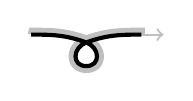
\begin{tikzpicture}
\draw[linestyle,fuzzright] 
(.7,0) to [out=180, in=20] (0,-.1)
	to [looseness=1.6, out=-160, in=180] (0,-.4)
	to [looseness=1.6, out=0, in=-20] (0,-.1)
	to [out=160, in=0] (-.7,0);
\begin{pgfonlayer}{background}
	\draw[->,outstyle] (.7,0) -- +(0:\arrowlength);
\end{pgfonlayer}
\end{tikzpicture}
\end{center}

\end{block}

\begin{block}{The Serre automorphism}
If $x$ is a fully dualizable object the Serre automorphism $\cS_x: x \rightarrow x$ is the image of the loop bordism.
\end{block}
\end{frame}

\begin{frame}{The belt bordism and Radford isomorphism}
\begin{block}{The square of the Serre}
If $n > 2$, we have that $\cS_x^2 \cong \mathrm{id}$.
\end{block}

\begin{block}{The belt bordism and Radford isomorphism}
In fact, we have an explicit distinguished trivialization of the square of the loop bordism, which we call the belt bordism.  Its image under a TFT is the Radford isomorphism $\cR_x$.

\begin{center}
\includegraphics[width=60mm]{../cobordism.png}
\end{center}

\end{block}
\end{frame}

\begin{frame}{Application to tensor categories}
\begin{defn}
Let ${}_{\langle\cF \rangle} \cC$ denote $\cC$ as a $\cC$--$\cC$ bimodule where the action is $$x \cdot c \cdot y = \cF(x) \otimes c \otimes y.$$  
\end{defn}

\begin{block}{Serre for $\mathcal{TC}$}
If $\cC$ is a finite tensor category then $$\cS_\cC \cong {}_{\langle\ldd{(-)}\rangle} \cC.$$
\end{block}

\begin{block}{Radford for $\mathcal{TC}$}
We have $\cR_\cC(1) = D$, and the structure of $\cR_\cC$ as a bimodule functor gives a natural isomorphism of tensor functors in Radford's theorem.
\end{block}
\end{frame}

\end{document}